%-----------------------------------------------------------------------------------------------
\documentclass[12pt,aspectratio=169]{beamer}
%-----------------------------------------------------------------------------------------------
\usepackage{pslatex}
\usepackage[greek,french,english,brazil]{babel} % last becomes the active one
\usepackage{ulem}
\renewcommand{\ULdepth}{3.0pt}
%-----------------------------------------------------------------------------------------------
\newcommand{\YA}{%
    \mbox{%
        Y\makebox[0pt][l]{\hspace{-0.178em}\raisebox{-0.00ex}{\scalebox{0.30}{E}}}%
        H\makebox[0pt][l]{\hspace{-0.010em}\raisebox{-0.00ex}{\scalebox{0.30}{O}}}%
        W\makebox[0pt][l]{\hspace{-0.245em}\raisebox{-0.00ex}{\scalebox{0.30}{A}}}%
        H%
    }%
}
%-----------------------------------------------------------------------------------------------
\newcommand{\ver}[1]{%
    \raisebox{0.50ex}{%
        \scalebox{1.1}{%
            \pmb{\textbf{\textcolor{BSpbg}{#1}}}%
        }%
    }%
}
%-----------------------------------------------------------------------------------------------
\newcommand{\QUOTE}[1]{%
    \par\noindent\hspace*{0.1\linewidth}%
    \begin{minipage}{0.8\linewidth}%
        \linespread{1.35}\large{#1}%
    \end{minipage}%
}
%-----------------------------------------------------------------------------------------------
\newcommand{\WIDEQUOTE}[1]{%
    \par\noindent\hspace*{0.02\linewidth}%
    \begin{minipage}{0.92\linewidth}%
        \linespread{1.25}\large{#1}%
    \end{minipage}%
}
%-----------------------------------------------------------------------------------------------
\newcommand{\RED}[1]{{\textcolor{TXred}{#1}}}
\newcommand{\ORA}[1]{{\textcolor{TXora}{#1}}}
\newcommand{\YEL}[1]{{\textcolor{TXyel}{#1}}}
\newcommand{\GRE}[1]{{\textcolor{TXgre}{#1}}}
\newcommand{\CYA}[1]{{\textcolor{TXcya}{#1}}}
\newcommand{\BLU}[1]{{\textcolor{TXblu}{#1}}}
\newcommand{\MAG}[1]{{\textcolor{TXmag}{#1}}}
\newcommand{\BRI}[1]{{\textcolor{BSpbg}{#1}}}   % Bright
%-----------------------------------------------------------------------------------------------
\newcommand{\ENtxt}[1]{\begin{otherlanguage}{english}{{#1}}\end{otherlanguage}}
\newcommand{\GRtxt}[1]{\begin{otherlanguage}{greek}{{#1}}\end{otherlanguage}}
\newcommand{\FRtxt}[1]{\begin{otherlanguage}{french}{{#1}}\end{otherlanguage}}
%-----------------------------------------------------------------------------------------------
\usetheme{CambridgeUS}
\usefonttheme{serif}
\usecolortheme{BShare1}
%-----------------------------------------------------------------------------------------------
\title{Estudo do \textit{Timing} em Mt 24.4--14}
\subtitle{Parte A --- O ``Fim'' em Mateus~24}
\author{Bíblia Share}
%\institute{Bíblia Share}
\date[{\tiny\tt{26 de fevereiro de 2022}}]{{\scriptsize\tt%
    \includegraphics[height=6.0mm]{res/cc/by-nc-88x31.pdf}\\[\smallskipamount]
    26 de fevereiro de 2022%\today
}}
%-----------------------------------------------------------------------------------------------
\begin{document}
%-----------------------------------------------------------------------------------------------
\logo{%
    \parbox{158mm}{% There's a 1mm gap on each side of the 160mm x 90mm slide logo line
    \mode<beamer>{%
        \hfill\includegraphics[height=9.0mm]{res/logo/BibliaShare.pdf}%
    }
    \mode<handout>{%
        \hfill\includegraphics[height=9.0mm]{res/logo/BibliaShare.pdf}%
    }
}}
%-----------------------------------------------------------------------------------------------
\begin{frame}
    \titlepage
\end{frame}
%%%-----------------------------------------------------------------------------------------------
%%\section{Verso Base}
%%%-----------------------------------------------------------------------------------------------

    \begin{frame}
        \QUOTE{%
            %-----!j 92 -i12
            \ver{(ARA) Mt~24.2}~%
            Ele, porém, lhes disse: \YEL{Não vedes tudo  isto?}  Em  verdade  vos  digo  que
            \YEL{não ficará aqui pedra sobre pedra que não seja derribada.}
        }
    \end{frame}

    \begin{frame}
        \QUOTE{%
            %-----!j 92 -i12
            \ver{(ARA) Mt~24.3}~%
            No monte das Oliveiras, achava-se Jesus assentado, quando se aproximaram dele os
            discípulos, \BRI{em particular}, e lhe pediram: Dize-nos  \YEL{quando  sucederão
            estas coisas} e \GRE{que sinal haverá da tua  vinda}  e  da  \MAG{consumação  do
            século}.
        }
    \end{frame}

    \begin{frame}
        \QUOTE{%
            %-----!j 92 -i12
            \ver{(ARA) Dn~9.20a}~%
            Falava eu ainda, e orava, e confessava o meu pecado e o pecado do \YEL{meu  povo
            de Israel} [...] \\[\bigskipamount]
            %-----!j 92 -i12
            \ver{(ARA) Dn~9.24}~%
            \GRE{Setenta semanas} estão \MAG{determinadas} sobre \YEL{o teu  povo}  e  sobre
            \ORA{a tua santa cidade}, para fazer cessar a transgressão,  para  dar  fim  aos
            pecados, para \BRI{expiar a iniquidade}, para  \BRI{trazer  a  justiça  eterna},
            para selar a visão e a profecia e para ungir o Santo dos Santos.
        }
    \end{frame}

    \begin{frame}
        \QUOTE{%
            %-----!j 92 -i12
            \ver{(ARA) Mt~24.15}~%
            \YEL{Quando}, pois, virdes \GRE{o  abominável  da  desolação}  de  que  falou  o
            \MAG{profeta Daniel}, no lugar santo (quem lê entenda),
        }
    \end{frame}

    \begin{frame}
        \QUOTE{%
            %-----!j 92 -i12
            \ver{(ARA) At~17.11}~%
            Ora, estes de \YEL{Bereia} eram \GRE{mais nobres} que os  de  Tessalônica;  pois
            receberam a palavra com toda a avidez, \MAG{examinando as  Escrituras  todos  os
            dias para ver se as coisas eram, de fato, assim}.
        }
    \end{frame}

    \begin{frame}
        \QUOTE{%
            %-----!j 92 -i12
            \ver{(ARA) Mt~24.15}~%
            \YEL{Quando}, pois, virdes \GRE{o  abominável  da  desolação}  de  que  falou  o
            \MAG{profeta Daniel}, no lugar santo (quem lê entenda), [...] \\[\bigskipamount]
            %-----!j 92 -i12
            \ver{(ARA) Mt~24.21}~%
            porque \YEL{nesse tempo} haverá \RED{grande tribulação}, como desde o  princípio
            do mundo até agora não tem havido e nem haverá jamais.
        }
    \end{frame}

    \begin{frame}
        \QUOTE{%
            %-----!j 92 -i12
            \ver{(ARA) Mt~24.15}~%
            \YEL{Quando}, pois, virdes \GRE{o  abominável  da  desolação}  de  que  falou  o
            \MAG{profeta Daniel}, no lugar santo (quem lê entenda), \\[\bigskipamount]
            %-----!j 92 -i12
            \ver{(ARA) Dn~9.27}~%
            Ele fará firme aliança com muitos, por uma semana; \YEL{na  metade  da  semana},
            fará cessar  o  sacrifício  e  a  oferta  de  manjares;  sobre  a  \GRE{asa  das
            abominações virá o assolador}, até que a destruição, que  está  determinada,  se
            derrame sobre ele.
        }
    \end{frame}

    \begin{frame}
        \QUOTE{%
            %-----!j 92 -i12
            \ver{(ARA) Mt~24.21}~%
            porque \YEL{nesse tempo} haverá \RED{grande tribulação}, como desde o  princípio
            do mundo até agora não tem havido e nem haverá jamais. \\[\bigskipamount]
            %-----!j 92 -i12
            \ver{(ARA) Dn~9.27}~%
            Ele fará firme aliança com muitos, por uma semana; \YEL{na  metade  da  semana},
            fará cessar  o  sacrifício  e  a  oferta  de  manjares;  sobre  a  \GRE{asa  das
            abominações virá o assolador}, até que a destruição, que  está  determinada,  se
            derrame sobre ele.
        }
    \end{frame}

    \begin{frame}
        \QUOTE{%
            %-----!j 92 -i12
            \ver{(A21) Mt~24.3}~%
            [...] seus discípulos  aproximaram-se  dele  em  particular,  dizendo:  Dize-nos
            \YEL{quando essas coisas acontecerão} e \GRE{que sinal haverá da tua vinda} e do
            \MAG{fim do mundo}. \\[\bigskipamount]
            %-----!j 92 -i12
            \ver{(ARC) Mt~24.3}~%
            [...] chegaram-se a ele os seus discípulos,  em  particular,  dizendo:  Dize-nos
            \YEL{quando serão essas coisas} e \GRE{que sinal  haverá  da  tua  vinda}  e  do
            \MAG{fim do mundo}?
        }
    \end{frame}

    \begin{frame}
        \QUOTE{%
            %-----!j 92 -i12
            \ver{(ARA) Ap~20.11}~%
            Vi um \BRI{grande trono branco} e \BRI{aquele que  nele  se  assenta},  de  cuja
            presença \YEL{fugiram} a \GRE{terra} e o \CYA{céu}, e \MAG{não  se  achou  lugar
            para eles}.
        }
    \end{frame}

    \begin{frame}
        \QUOTE{%
            %-----!j 92 -i12
            \ver{(ARA) Mt~24.3}~%
            No monte das Oliveiras, achava-se Jesus assentado, quando se aproximaram dele os
            discípulos, \BRI{em particular}, e lhe pediram: Dize-nos  \YEL{quando  sucederão
            estas coisas} e \GRE{que sinal haverá da tua  vinda}  e  da  \MAG{consumação  do
            século}.
        }
    \end{frame}

    \begin{frame}
        \QUOTE{%
            %-----!j 92 -i12
            \ver{(SBL) Mt~24.3}~%
            \GRtxt{Καθημένου δὲ αὐτοῦ ἐπὶ τοῦ Ὄρους τῶν Ἐλαιῶν  προσῆλθον  αὐτῷ  οἱ  μαθηταὶ
            κατ’ ἰδίαν λέγοντες· Εἰπὸν ἡμῖν \YEL{πότε ταῦτα ἔσται}, καὶ \GRE{τί  τὸ  σημεῖον
            τῆς σῆς παρουσίας} καὶ \MAG{συντελείας τοῦ αἰῶνος}}.
            % THANKS to https://jwodder.github.io/kbits/posts/unicode-latex/
        }
    \end{frame}

    \begin{frame}
        \begin{center}
            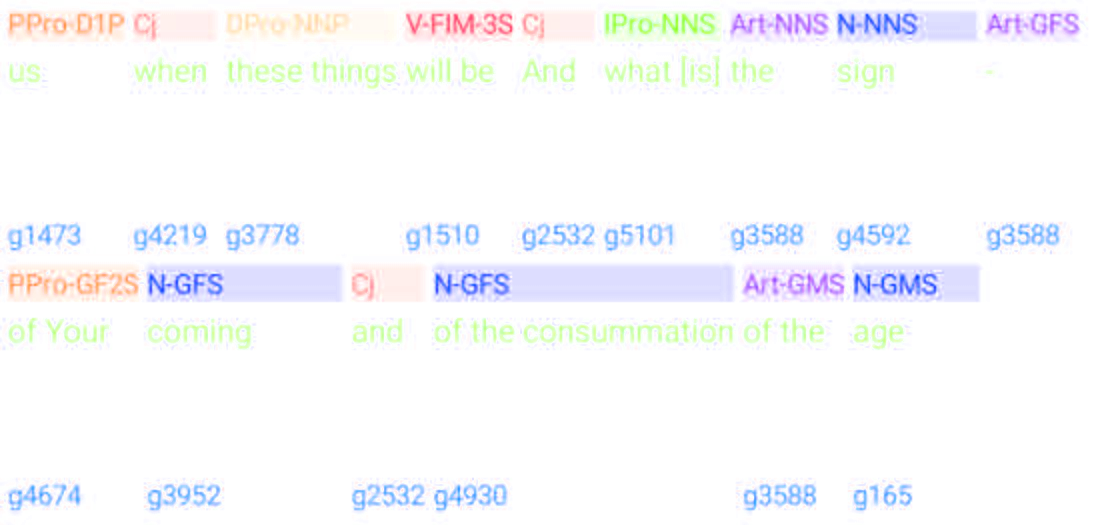
\includegraphics[width=128mm]{fig/Mt24-Greek-Crop-Alpha.png}
        \end{center}
    \end{frame}

    \begin{frame}
        \QUOTE{%
            %-----!j 92 -i12
            \ver{(ARA) Mt~25.46}~%
            E irão estes para o \RED{castigo eterno}, porém  os  justos,  para  a  \GRE{vida
            eterna}.
        }
    \end{frame}

    \begin{frame}
        \WIDEQUOTE{%
            %-----!j 92 -i12
            \ver{(ARA) Ap~19.19,20}~%
            E vi a \YEL{besta} e os reis da terra,  com  os  seus  exércitos,  [...]  contra
            \BRI{aquele que estava montado no  cavalo}  e  contra  o  seu  exército.  Mas  a
            \YEL{besta} foi aprisionada, e com ela o \ORA{falso profeta} que  [...]  seduziu
            aqueles que receberam a \MAG{marca da besta} e eram os  adoradores  da  \GRE{sua
            imagem}. \\[\bigskipamount]
            %-----!j 92 -i12
            \ver{(ARA) Ap~20.4}~%
            Vi ainda [...] tantos  quantos  não  adoraram  a  \YEL{besta},  nem  tampouco  a
            \GRE{sua imagem},  e  não  receberam  a  \MAG{marca  na  fronte  e  na  mão};  e
            \BRI{viveram e reinaram com Cristo durante mil anos}.
        }
    \end{frame}

    \begin{frame}
        \WIDEQUOTE{%
            %-----!j 92 -i12
            \ver{(ARA) Ap~19.19,20}~%
            E vi a \YEL{besta} e os reis da terra,  com  os  seus  exércitos,  [...]  contra
            \BRI{aquele  que  estava  montado  no  cavalo}  [...]  Mas  a  \YEL{besta}   foi
            aprisionada, e com ela o \ORA{falso profeta}  [...]  Os  \YEL{do}\ORA{is}  foram
            lançados vivos dentro do lago de fogo [...]
            \\[\bigskipamount]
            %-----!j 92 -i12
            \ver{(ARA) Ap~20.2,4}~%
            Ele prendeu o \RED{dragão}, a \RED{antiga  serpente},  que  é  o  \RED{diabo}  e
            \RED{Satanás}, e amarrou-o por mil anos. [...] Vi ainda [...] tantos quantos não
            adoraram a \YEL{besta}, nem tampouco a  \GRE{sua  imagem},  e  não  receberam  a
            \MAG{marca na fronte e na mão}; e \BRI{viveram e reinaram com Cristo durante mil
            anos}.
        }
    \end{frame}

    \begin{frame}
        \QUOTE{%
            %-----!j 92 -i12
            \ver{(ARA) Ap~20.4}~%
            Vi também tronos, e nestes sentaram-se aqueles aos quais foi dada autoridade  de
            julgar. Vi ainda as almas dos decapitados por causa do testemunho de Jesus,  bem
            como por causa da palavra de Deus, tantos quantos  não  adoraram  a  besta,  nem
            tampouco a sua  imagem,  e  não  receberam  a  marca  na  fronte  e  na  mão;  e
            \BRI{viveram e \textbf{reinaram com Cristo durante mil anos}}.
        }
    \end{frame}

    \begin{frame}
        \QUOTE{%
            %-----!j 92 -i12
            \ver{(ARA) 2Ts~2.7,8}~%
            Com efeito, o \RED{mistério da iniquidade} já opera e \YEL{aguarda somente}  que
            \GRE{seja afastado} aquele que \GRE{agora o detém}; \MAG{então, será,  de  fato,
            revelado} o \RED{iníquo}, a quem o Senhor Jesus matará com o sopro de sua boca e
            o destruirá pela manifestação de sua vinda.
        }
    \end{frame}

    \begin{frame}
        \QUOTE{%
            %-----!j 92 -i12
            \ver{(ARA) Dt~18.21,22}~%
            Se disseres no  teu  coração:  \YEL{Como  conhecerei  a  palavra  que  o  Senhor
            \textbf{não} falou}? \MAG{\textbf{Sabe que}}, quando esse \ORA{profeta falar  em
            nome do Senhor}, e a palavra dele se \GRE{\textbf{não  cumprir,  nem  suceder}},
            \CYA{\textbf{como profetizou}}, \MAG{esta é palavra  que  o  Senhor  \textbf{não
            disse}}; com \ORA{soberba}, a falou o tal profeta; \ORA{não tenhas temor dele}.
        }
    \end{frame}

    \begin{frame}
        \QUOTE{%
            %-----!j 92 -i12
            \ver{(ARA) Js~23.14}~%
            Eis que,  já  hoje,  sigo  pelo  caminho  de  todos  os  da  terra;  e  vós  bem
            \YEL{\textbf{sabeis} de todo o vosso  coração  e  de  toda  a  vossa  alma}  que
            \GRE{\textbf{nem uma só promessa caiu de todas as boas palavras}} que  falou  de
            vós o Senhor, vosso Deus; \MAG{\textbf{todas  vos  sobrevieram,  nem  uma  delas
            falhou}}.
        }
    \end{frame}

    \begin{frame}
        \QUOTE{%
            %-----!j 92 -i12
            \ver{(ARA) Ap~20.4}~%
            e \BRI{viveram e \textbf{reinaram com Cristo durante mil anos}}.
        }
    \end{frame}

    \begin{frame}
        \QUOTE{%
            %-----!j 92 -i12
            \ver{(ARA) Ap~20.11}~%
            Vi um \BRI{grande trono branco} e \BRI{aquele que  nele  se  assenta},  de  cuja
            presença \YEL{fugiram} a \GRE{terra} e o \CYA{céu}, e \MAG{não  se  achou  lugar
            para eles}.
        }
    \end{frame}

    \begin{frame}
        \QUOTE{%
            %-----!j 92 -i12
            \ver{(A21) Gn~1.7,8}~%
            E Deus fez o \YEL{\textbf{firmamento}} e  \ORA{separou}  as  águas  que  estavam
            debaixo do firmamento das que estavam por cima dele. [...] E \YEL{ao  firmamento
            Deus chamou \textbf{céu}}. \\[\bigskipamount]
            %-----!j 92 -i12
            \ver{(A21) Gn~1.16,17}~%
            E Deus fez os \CYA{dois grandes luminares}: o luminar maior para governar o  dia
            e o  menor  para  governar  a  noite;  \MAG{fez  também  as  estrelas}.  E  Deus
            \GRE{\textbf{os colocou no firmamento} celeste} para iluminar a terra,
        }
    \end{frame}


    \begin{frame}
        \QUOTE{%
            %-----!j 92 -i12
            \ver{(ARA) Mt~24.3}~%
            No monte das Oliveiras, achava-se Jesus assentado, quando se aproximaram dele os
            discípulos, \BRI{em particular}, e lhe pediram: Dize-nos  \YEL{quando  sucederão
            estas coisas} e \GRE{que sinal haverá da tua  vinda}  e  da  \MAG{consumação  do
            século}. \\[\bigskipamount]
            %-----!j 92 -i12
            \ver{(ARA) Mt~25.46}~%
            E irão estes para o \RED{castigo eterno}, porém  os  justos,  para  a  \GRE{vida
            eterna}.
        }
    \end{frame}

    \begin{frame}
        \QUOTE{%
            %-----!j 92 -i12
            \ver{(ARA) Mt~25.31--33}~%
            \YEL{Quando \textbf{vier}} o Filho do Homem na sua majestade e  todos  os  anjos
            com ele,  então,  se  assentará  no  \GRE{trono  da  sua  glória};  e  todas  as
            \CYA{nações serão reunidas em  sua  presença},  e  ele  \ORA{separará}  uns  dos
            outros, como o pastor separa dos cabritos as ovelhas; e porá as  ovelhas  à  sua
            \BLU{direita}, mas os cabritos, à \RED{esquerda};
        }
    \end{frame}

    \begin{frame}
        \QUOTE{%
            %-----!j 92 -i12
            \ver{(ARA) Jl~3.1,2,17}~%
            Eis que, naqueles dias e naquele tempo, em que mudarei a sorte de  \YEL{Judá}  e
            de \ORA{Jerusalém}, congregarei \CYA{todas as  nações}  e  as  farei  descer  ao
            \GRE{vale de Josafá}; e ali \RED{entrarei em juízo contra elas} por causa do meu
            povo e da minha herança, Israel. [...] eu sou o  \BRI{Senhor,  vosso  Deus,  que
            habito em  Sião,  meu  santo  monte};  e  \ORA{Jerusalém  \textbf{será}  santa};
            estranhos não passarão mais por ela.
        }
    \end{frame}

    \begin{frame}
        \QUOTE{%
            %-----!j 92 -i12
            \ver{(ARA) Mt~25.46}~%
            E irão estes para o \RED{castigo eterno}, porém  os  justos,  para  a  \GRE{vida
            eterna}. \\[\bigskipamount]
            %-----!j 92 -i12
            \ver{(ARA) Jl~3.17}~%
            [...] eu sou o \BRI{Senhor, vosso Deus, que habi\-to em Sião, meu santo monte};  e
            \ORA{Jerusalém \textbf{será} santa}; estranhos não passarão mais por ela.
            $\qquad$(\GRE{Milênio}) \\[2\bigskipamount]
            %-----!j 92 -i12
            \YEL{\only<2>{$\rightharpoondown$ O Milênio \textbf{é} o início da vida eterna!}}
        }
    \end{frame}

    \begin{frame}
        \QUOTE{%
            %-----!j 92 -i12
            \ver{(ARA) Mt~24.4,5}~%
            [...] Vede que  ninguém  vos  \RED{\textbf{engane}}.  Porque  \YEL{virão  muitos
            \textbf{em meu nome}} [...] e \RED{\textbf{enganarão a muitos}}.
        }
    \end{frame}

    \begin{frame}
        \large
        %-----!j 96 -i8
        O \BRI{\textbf{engano}}, sendo  o  sinal  mais  frequentemente  citado  pelo  Senhor  em
        Mateus~24 e estando em plena operação nos dias  dos  Atos  dos  Apóstolos  (ver,  p.ex.:
        At~13.10), nas muitas heresias introduzidas na história da igreja, e nos tempos do  fim,
        deixa   \BRI{\textbf{mais   que   evidente}}   que   Satanás   ---   o   enganador   ---
        \BRI{\textbf{segue solto}} desde o Século~I até a Segunda Vinda  de  Cristo,  falada  em
        Apocalipse~19, indicando que nem (i)~a ``era da igreja'', nem  (ii)~a  tribulação  podem
        ser considerados ``reino de Deus'', fazendo do \BRI{\textbf{Milênio}}  de  Apocalipse~20
        uma época seguramente \BRI{\textbf{distinta (e futura!)}}.
    \end{frame}

    \begin{frame}
        \QUOTE{%
            %-----!j 92 -i12
            \ver{(ARA) Dn~2.27}~Respondeu Daniel na presença do rei e disse: O mistério  que
            o rei exige, nem encantadores, nem magos nem astrólogos o podem revelar ao  rei;
            \ver{28}~\MAG{mas há um Deus no céu}, o qual revela os mistérios, pois fez saber
            ao rei Nabucodonosor \YEL{o que há de ser nos últimos dias}. \GRE{O teu sonho  e
            as visões da tua cabeça, quando estavas no teu leito, são estas:}
        }
    \end{frame}

    \begin{frame}
        \QUOTE{%
            %-----!j 92 -i12
            \ver{(ARA) Dn~2.29}~\GRE{Estando  tu,  ó  rei,  no   teu   leito,   surgiram-te
            pensamentos a respeito do que há de ser depois disto}.  \MAG{Aquele,  pois,  que
            revela mistérios} te revelou \YEL{o que há de ser}.  \ver{30}~E  a  mim  me  foi
            revelado este mistério, não porque haja em mim mais sabedoria do que em todos os
            viventes, mas para que a interpretação se fizesse  saber  ao  rei,  e  para  que
            entendesses as \GRE{cogitações da tua mente}.
        }
    \end{frame}

    \begin{frame}
        \QUOTE{%
            %-----!j 92 -i12
            \ver{(ARA) Dn~2.31}~Tu, ó  rei,  estavas  vendo,  e  eis  aqui  \BRI{uma  grande
            estátua}; esta, que era imensa e de extraordinário esplendor, estava \BRI{em pé}
            diante de ti; e a sua \BRI{aparência era terrível}. \ver{32}~A \BRI{cabeça}  era
            de fino ouro, o \BRI{peito e os braços}, de prata, o \BRI{ventre e os  quadris},
            de bronze; \ver{33}~as \BRI{pernas}, de ferro, os \BRI{pés}, em parte, de ferro,
            em parte, de barro.
        }
    \end{frame}

    \begin{frame}
        \QUOTE{%
            %-----!j 92 -i12
            \ver{(ARA) Dn~2.34}~Quando estavas olhando, \GRE{uma \textbf{pedra}} foi cortada
            \GRE{sem auxílio de mãos}, \ORA{feriu} a estátua nos pés de ferro e de  barro  e
            os \ORA{esmiuçou}. \ver{35}~Então, foi juntamente esmiuçado o ferro, o barro,  o
            bronze, a prata e o ouro, os quais se fizeram como a palha das eiras no estio, e
            o  vento  os  levou,  e   deles   não   se   viram   mais   vestígios.   Mas   a
            \GRE{\textbf{pedra}} que  feriu  a  estátua  se  tornou  em  \GRE{\textbf{grande
            montanha}}, que \CYA{encheu toda a \textbf{terra}}.
        }
    \end{frame}

    \begin{frame}
        \QUOTE{%
            %-----!j 92 -i12
            \ver{(ARA) Is~2.10}~Vai, entra nas rochas e esconde-te no pó, ante o \MAG{terror
            do Senhor} e a \YEL{glória da sua  majestade}.  \ver{11}~Os  olhos  altivos  dos
            homens serão abatidos, e a sua altivez será humilhada;  \MAG{só  o  Senhor  será
            exaltado naquele dia}. \ver{12}~Porque o \GRE{Dia do Senhor dos Exércitos}  será
            \RED{contra} todo soberbo e altivo e \RED{contra} todo  aquele  que  se  exalta,
            para que seja abatido; \ver{13}~\RED{contra} todos os cedros do  Líbano,  altos,
            mui elevados; e \RED{contra} todos os carvalhos de Basã;
        }
    \end{frame}

    \begin{frame}
        \QUOTE{%
            %-----!j 92 -i12
            \ver{(ARA) Is~2.14}~\RED{contra} todos os montes altos e \RED{contra}  todos  os
            outeiros elevados; \ver{15}~\RED{contra} toda torre  alta  e  \RED{contra}  toda
            muralha firme; \ver{16}~\RED{contra} todos os navios de  Társis  e  \RED{contra}
            tudo o que é belo à vista. \ver{17}~A arrogância do homem será abatida, e a  sua
            altivez será humilhada; \MAG{só o Senhor será exaltado naquele dia}.
        }
    \end{frame}

    \begin{frame}
        \QUOTE{%
            %-----!j 92 -i12
            \ver{(ARA) Is~2.18}~Os \RED{ídolos serão de todo destruídos}. \ver{19}~Então, os
            homens se meterão nas cavernas das  rochas  e  nos  buracos  da  terra,  ante  o
            \MAG{terror do Senhor} e a \YEL{glória da sua majestade}, quando ele se levantar
            para espantar a terra. \ver{20}~Naquele dia, os homens lançarão às  toupeiras  e
            aos morcegos os seus \RED{ídolos} de prata e os seus \RED{ídolos} de  ouro,  que
            fizeram para ante eles se prostrarem,
        }
    \end{frame}

%%%-----------------------------------------------------------------------------------------------
%%\section{Referências}
%%%-----------------------------------------------------------------------------------------------

%%    %------------------------------------------------------------------------------------------
%%    \begin{frame}[allowframebreaks]{Referências -- }
%%        \bibliographystyle{unsrt}
%%        \setbeamertemplate{bibliography item}{\insertbiblabel}
%%        \bibliography{bibfile.bib}
%%    \end{frame}
%%    %------------------------------------------------------------------------------------------

%-----------------------------------------------------------------------------------------------
\end{document}
%-----------------------------------------------------------------------------------------------
